\documentclass{article}

\usepackage{amsmath}
\usepackage{amsfonts}
\usepackage[dvips]{graphicx}

\usepackage{natbib}
\usepackage{url}

\bibliographystyle{apa}

\newenvironment{eqnnon}{\begin{equation}}{\end{equation}}

\begin{document}

\title{Solving for multi-class: a synthesis\\(manuscript in progress)}

\author{Peter Mills\\\textit{peteymills@hotmail.com}}

\maketitle

\section{Introduction}

Many statistical classifiers can only discriminate between two classes.
Common examples include linear classifiers such as perceptrons and
logistic regression classifiers \citep{Michie_etal1994} as well as extensions
of these methods such as support vector machines (SVM) \citep{Mueller_etal2001} and 
piecewise linear classifiers \citep{Mills2011, Bagirov2005}.
There are many possible ways of extending a binary classifier to deal
with multi-class classification and the options increase exponentially
with the class labels.
Moreover, the best method may well depend on the type of problem
\citep{Dietterich_Bakiri1995,Allwein_etal2000}.

The goal of this paper is not only to provide a summary of the
best methods of solving for multiclass, but to synthesize
these ideas into a comprehensive framework whereby a multi-class problem
can be solved using a broad array of configurations for the binary
classifiers. 
This includes solving for the multi-class conditional probabilities.

\subsection{Definition of the problem}

\label{description}

In a statistical classication problem we are given a set of ordered pairs, 
$\lbrace \vec x_j : y_j \rbrace$, of {\it training data},
where the vector, $\vec x_j$, is the location of the {\it sample} in 
the {\it feature space},
$y_j \in [1..n_c]$ is the class of the sample,
$n_c$ is the number of classes,
and the classes are
distributed according to an unknown conditional distribution,
$P(c | \vec x)$ with $c \in [1..n_c]$ the class label and $\vec x$ the location
in feature space.

Given an arbitrary {\it test point}, $\vec x$, 
we wish to estimate $P(c | \vec x)$, however we only have
the means to estimate some binary component of it, that is we have a 
set of binary classifiers, 
each returning a {\it decision function}, $r_i(\vec x)$.
In this paper we assume that the decision function 
returns estimates of the difference in conditional probabilities:
\begin{equation}
	r_i(\vec x) \approx p_i(+1|\vec x) - p_i(-1|\vec x)
\end{equation}
where $p_i(c|\vec x)$ is the conditional probability of the $i$th
binary classifier.
The decision function is trained using the same type of ordered pairs as
above except that the classes can only take on one of two values,
which for convenience are chosen as either $-1$ or $+1$, 
that is, $y_{ij} \in \lbrace -1, +1 \rbrace$.

The problem under consideration in this review is, first,
how can we partition the classes, $\lbrace y_i \rbrace$, for each binary
classifier?
That is we want to create a mapping of the form:
\begin{equation}
	y_{ij} (y_j) = \left \lbrace  \begin{array}{lr}
-1 & | y_j \in C_i^+ \\
+1 & | y_j \in C_i^-
\end{array}
\right .
\end{equation}
where $y_{ij}$ is the class value of $j$th sample of the transformed data 
for trainng the $i$th binary classifier and 
$C_i^+ \subset \lbrace 1..n_c \rbrace$ is the set of class labels from the original set,
$\lbrace 1..n_c \rbrace$, that map to $+1$ while
$C_i^- \subset \lbrace 1..nc \rbrace$ is the set of classes that map to $-1$.

And second, once we have partitioned the classes
and trained the binary classifers,
how do we solve for the conditional probabilities, $P(c|\vec x)$?
Alternatively, we might be able to solve directly for the most likely class:
%how do we solve for the most likely class, 
\begin{equation}
	c(\vec x)=\arg \max_i P(i | \vec x)
\end{equation}

%given a test point, $\vec x$,
%or alternatively, directly for $P(c | \vec x)$ where $c$ is either the most likely class
%or else can be any of the classes, $c \in [1,n_c]$?
%--that is all of the conditional probabilities 
%or just that of the ``winning'' class?


\section{Nonhierarchical multi-class classification}

In {\it non-hierarchical} multi-class classification, we solve for the
classes or probabilities of the multi-class problem all at once:
all the binary classifiers are used in the solution and the result of
one binary classifier does not determine the use of any of the others.
Using the notation provided in Section \ref{description}, 
we can write a system of equations relating
the multi-class conditional probabilities to the decision
functions:
\begin{equation}
	r_i(\vec x) = \frac{\sum_{j=1}^{n_i^+} P(c_{ij}^+|\vec x) - \sum_{j=1}^{n_{i}^-} P(c_{ij}^-|\vec x)}{\sum_{j=1}^{n_i^-} P(c_{ij}^-|\vec x) + \sum_{j=1}^{n_i^+} P(c_{ij}^+|\vec x)}
	\label{decision_function}
\end{equation}
where 
$c_{ij}^- \in C_i^-$,
$c_{ij}^+ \in C_i^+$,
$n_i^-$ is the number of class labels on the negative side of
the $i$th partition,
and $n_i^+$ is the number of class labels on the positive side of
the $i$th partition

It's more natural to describe the problem using a
{\it coding matrix}, $A$, 
which is structured such that
$a_{ij} \in \lbrace -1, 0, 1 \rbrace$, 
where $i$ enumerates the binary classifier and
$j$ enumerates the class of the multi-class problem.
In other words, if $a_{ij}$ is $-1$/$+1$, we would assign each of the $j$th class
labels in the training data a value of $-1$/$+1$ when training the $i$th
binary classifier. If the value is $0$, the $j$th class label is excluded.
\citep{Dietterich_Bakiri1995,Windeatt_Ghaderi2002}

The non-zero elements of $A$ are:
\begin{eqnarray}
	a_{ic_{ik}^-} & = & -1 | ~k = [1..n_{c_i^-}]\\
a_{ic_{ik}^+} & = & +1 | ~k=[1..n_{c_i^+}]
\end{eqnarray}

%We can relate the multi-class probabilities to the output of the 
%binary classifiers as follows:
We can rewrite Equation (\ref{decision_function}) using the decision
matrix as follows:
\begin{equation}
	\frac{\sum_{j=1}^{n_c} a_{ij} p_j}{\sum_{j=1}^{n_c} |a_{ij}| p_j} = r_i
	\label{non_hier}
\end{equation}
where $\vec p=\lbrace p_i | i=[1..n_c]\rbrace$, 
is a vector of multi-class conditional probabilities, $p_i=P(i|\vec x)$, 
$n_c$ is the number of classes,
$\vec r=\lbrace r_i| i=[1..n_p]\rbrace$ 
is the vector of decision functions,
and
$n_p$ is the number of partitions.

Some rearrangement shows that
we can solve for the probabilities, $\vec p$, via matrix inversion:
\begin{eqnarray}
	Q \vec p & = & \vec r \label{basic_system}\\
	%q_{ij} & = & a_{ij} + \delta(a_{ij}) r_i \\
	q_{ij} & = & a_{ij} + (1-|a_{ij}|) r_i 
	\label{matrix_equation2}
\end{eqnarray}
%and $\delta$ is the Kronecker delta.
Note that $Q$ reduces to $A$ if $A$ contains no zeroes \citep{Kong_Dietterich1997}.
The case of a coding matrix that contains no zeroes, that is all the partitions divide up all the
classes rather than a subset, will be called the {\it strict} case.
From a computational perspective, in the strict case,
$Q$ must be regenerated for every new test point or value of $\vec r$ 
whereas in the non-strict case, $A$ can be inverted or decomposed and then
applied to every subsequent value of $\vec r$.

Because the decision functions, $\vec r$, are not estimated perfectly,
the final probabilities may need to be constrained and the inverse
problem solved via minimization:
\begin{equation}
	\vec p = \arg \min_{\vec v} | Q \vec v - \vec r | \label{minimization_problem}
\end{equation}
subject to:
\begin{eqnarray}
	\sum_{i=1}^{n_c} p_i & = & 1 \label{normalization}\\
	p_i & \ge & 0 \label{nonnegative}
\end{eqnarray}
where straight brackets, $||$, denotes a vector norm which  
in this case is the Euclidian or $L^2$ norm.

The class of the test point is determined through maximum likelihood:
\begin{equation}
	c = \arg \max_i p_i
\end{equation}

\subsection{Basic inverse solution}

Equation (\ref{minimization_problem}) can be solved via the normal
equation:
\begin{equation}
	Q^T Q \vec p = Q^T \vec r
	\label{normal_equation}
\end{equation}
Because the binary probability estimates in $\vec r$ are rarely perfect, however,
in many cases the constraints in (\ref{normalization}) and (\ref{nonnegative}) will not be satisfied. 
Therefore, for most applications, either the results will need to be adjusted, likely reducing accuracy, or the problem constrained.

It is straightforward to incorporate the normalization constraint in (\ref{normalization}) into the problem. 
There are at several ways of doing this. The most
obvious is to write one probability in terms of the others:
\begin{equation}
	p_k = 1 - \sum_{i|i \ne k} p_i
	\label{reduce_dimension1}
\end{equation}
And solve the following, reduced dimensional linear system:
\begin{equation}
	\sum_j (q_{ij} - q_{ik} ) p_j = r_i - q_{ik}
	\label{reduce_dimension2}
\end{equation}
A more symmetric method is the Lagrange multiplier which will be
derived in Section \ref{one_vs_one}.
\citet{Hanson_Lawson1995} discuss at least two other methods of
enforcing equality constraints on linear least squares problems.

Since they are inequality constraints, those in (\ref{nonnegative}) are
harder to enforce and details  will be left to a later section.
\citet{Hanson_Lawson1995} outline several methods of applying equality
constraints to least squares. Moreover when a Lagrange multiplier is added
to the one-versus-one method, a basics matrix inverse generates probability
estimates that obey the inequality constraints. See below.

\subsection{Voting solution}

In many other texts \citep{Allwein_etal2000, Hsu_Lin2002, Dietterich_Bakiri1995},
the class of the test point is determined by how close $\vec r$
is to each of the columns in $A$:
\begin{equation}
	c = \arg \min_i |\vec a^{(i)} - \vec r|^2
\end{equation}
where $\vec a^{(i)}$ is the $i$th column of $A$.
For the norm, $||$, Hamming distance is
frequently used, which is the number of bits that must be changed
in a binary number in order for it to match another binary number.
This assumes that each decision function returns only one of two values: 
$r_i \in \lbrace -1, +1 \rbrace$.
If the coding matrix is strict, then:
\begin{equation}
	|\vec a^{(j)} - \vec r| = \sum_i \delta_{a_{ij} r_i}
\end{equation}
where $\delta$ is the Kronecker delta.
\citet{Allwein_etal2000} 
tailor the matric on the basis of the binary classifier used, each of which
will return a different type of continuous decision function 
(that doesn't represent the difference in conditional probabilities).

Here we are assuming that the decision functions return an approximation of the 
difference in conditional probabilities of the binary classifier.
In this case a more natural choice of metric is the Euclidian. Expanding:
\begin{equation}
	c = \arg \min_i \left \lbrace |\vec a^{(i)}|^2 - 2 \vec a^{(i)} \cdot \vec r + |\vec r|^2 \right \rbrace
\end{equation}
The length of $\vec r$ is independent of $i$, hence it can be eliminated from the expression.
For the strict case, the length of each column will also be constant at $|\vec a^{(i)}|=\sqrt{n_p}$.
Even for the non-strict case, we would expect the column lengths to be close for typical coding 
matricesr; for instance, the column lengths are equal in the one-versus-one case.
Eliminating these two terms produces a {\it voting} solution:
\begin{equation}
	c = \arg \max A^T \vec r
\end{equation}
That is, if the sign of $r_i$ matches the $i$th element of the column, then a vote is cast 
in proportion to the size of $r_i$ for the class label corresponding to the column number.

A voting solution can be used for any coding matrix and 
is especially appropriate if each $r_i$ returns only $-1$ or $+1$.  
The LIBSVM libary, for instance, uses a one-versus-one arrangement with a voting
solution if probabilities are not required \citep{Chang_Lin2011}.
The disadvantage of a voting solution is
that it does not return estimates of the probabilities.

\section{Common coding matrices}

There are a number of standard, symmetric coding matrices that are commonly used
to solve for multi-class.
These include ``one-versus-the-rest'', ``one-versus-one'',
as well as error-correcting coding matrices such as orthogonal and
random.
We discuss each of these in turn and
use them to demonstrate how to solve for the
conditional probabilities while enforcing the constraints,
expanding out to the general solution for ``error-correcting-codes.''

\subsection{One-versus-the-rest}

Common coding matrices include ``one-versus-the-rest'' in which
we take each class and train it against the rest of the
classes.
For $n_c=4$ it works out to:
\begin{equation}
A = 
\begin{bmatrix}
1 & -1 & -1 & -1 \\
-1 & 1 & -1 & -1 \\
-1 & -1 & 1 & -1 \\
-1 & -1 & -1 & 1
\end{bmatrix}
\end{equation}
or in the general case:
\begin{equation}
	a_{ij}=2 \delta_{ij}-1
\end{equation}
where $\delta$ is the Kronecker delta.

Probabilities for the one-versus-the-rest can be solved for directly by
simply writing out one side of the equation:
\begin{equation}
	p_i = (r_i + 1)/2
\end{equation}
The normalization constraint, (\ref{normalization}), can be enforced 
through the use of a Lagrange multiplier. See next section.

\subsection{One-versus-one}

\label{one_vs_one}

In a ``one-versus-one'' solution, we train each class against
every other class. For $n_c=4$:
\begin{equation}
A = 
\begin{bmatrix}
-1 & 1 & 0 & 0 \\
-1 & 0 & 1 & 0 \\
-1 & 0 & 0 & 1 \\
0 & -1 & 1 & 0 \\
0 & -1 & 0 & 1 \\
0 & 0 & -1 & 1
\end{bmatrix}
\end{equation}
The one-versus-one solution is used in LIBSVM \citep{Chang_Lin2011}.

Consider the following rearrangement of (\ref{non_hier}):
\begin{eqnarray}
	Q \vec p & = & \vec 0 \\
	q_{ij} & = & a_{ij} - r_i |a_{ij}|
\end{eqnarray}
We can include the normalization constraint, (\ref{normalization}), via
a Lagrange multiplier:
\begin{equation}
	\min_{\vec p, \lambda} \left \lbrace | Q \vec p | + \lambda(\vec 1 \cdot \vec p - 1) \right \rbrace
\end{equation}
which produces the following linear system:
\begin{eqnarray}
	\sum_k q_{ki} q_{kj} p_j + \lambda & = & 0 \\
	\sum_j p_j & = & 1
\end{eqnarray}
With this solution for a 1-vs-1 coding matrix, it can be shown that the
inequality constraints in (\ref{nonnegative}) are always satisfied
\citep{Wu_etal2004}.

\citet{Hsu_Lin2002} find that the one-vs.-one method is more accurate
for support vector machines (SVM) than either
error-correcting codes or one-vs.-the-rest.

\subsection{Orthogonal coding matrix}

\label{orthogonal}

An error correcting coding matrix is simply an arbitrary one.
This is often random, but may also be carefully designed 
\citep{Crammer_Singer2002}.
To maximize the accuracy of an error-correcting coding matrix, 
\citet{Allwein_etal2000} and \citet{Windeatt_Ghaderi2002} show that
the distance between each of the columns, $| \vec a^{(i)} - \vec a^{(j)} |$, 
should be as large as possible,
where $\vec a^({i})$ is the $i$th column of the matrix $A$ and $i \ne j$. 
If we take the upright brackets once again to be a
Euclidian metric and assume that $A$ is ``strict'' then this 
reduces to minimizing the absolute value of the dot product,
$|\vec a^{(i)} \cdot \vec a^{(j)}|$.
The absolute value is used because a pair of columns that are the same except 
for a factor of -1 are degenerate.

In other words, 
%if the number of rows is equal to the number of classes, 
the optimal coding matrix will be orthogonal, $A^T A = n_p I$, where $I$ is
the $[n_c\times n_c]$ identity matrix. 
Thus the voting solution and the (unconstrained) matrix 
inverse will be equivalent. Orthogonal, ``strict'' coding matrices 
are not hard to construct for certain class sizes, for instance:
\begin{equation}
A = 
\begin{bmatrix}
1 & -1 & -1 & -1 \\
-1 & 1 & 1 & 1 \\
-1 & -1 & -1 & 1 \\
-1 & -1 & 1 & -1
\end{bmatrix}
\end{equation}
Orthogonal coding matrices for the non-strict case are even easier to
construct, but the voting solution does not correspond to the inverse solution.

The orthogonality property allows us to reduce the minimization problem 
in (\ref{minimization_problem}) to something much simpler:
\begin{equation}
	\arg \min_{\vec p} | \vec p - \vec p_0 |
\end{equation}
where $\vec p_0 = A^T \vec r/m$ with the constraints in (\ref{normalization}) and
(\ref{nonnegative}) remaining the same.
Because the system has been rotated and expanded, the non-negativity 
constraints in (\ref{nonnegative}) remain orthogonal, meaning they are 
independent: enforcing one by setting one of the probabilities to zero, 
$p_k=0$ for example, shouldn't otherwise affect the solution.
This still leaves the normalization constraint in (\ref{normalization}):
the problem, now strictly geometrical, is comprised of finding the point nearest $p_0$ on the diagonal hyper-surface that bisects the unit hyper-cube.

Briefly, we can summarize the algorithm as follows:
1. move to the nearest point that satisfies the normalization constraint,
(\ref{normalization}); 2. if one or more of the probabilities is negative,
move to the nearest point that satisfies both 
the normalization constraint
and the non-negativity constraints, (\ref{nonnegative}), for the negative probabilities;
3. repeat step 2.
More formally, let $\vec 1$ be a vector of all $1$'s:
\begin{itemize}
	\item $i=1$; $n_1=n$
	\item while $\exists k \, p_{ik} < 0 \lor \vec p_i \cdot \vec 1 \ne 1$:
	\begin{itemize}
		\item if $\vec p_i \cdot \vec 1 \ne 1$ then 
		$\vec p_{i+1} = \vec p_i + (\vec p_i \cdot \vec 1 - 1)/n_i$
		\item let $K$ be the set of $k$ such that $p_{i+1,k} < 0$
		\item for each $k$ in $K$:
		\begin{itemize}
			\item $p_k=0$
			\item Remove $k$ from the problem
		\end{itemize}
		\item $n_{i+1}=n_i-|K|$
		\item $i=i+1$
	\end{itemize}
\end{itemize}

Note that resultant direction vectors for each step form an orthogonal set.
For instance, suppose $n_1=4$ and after enforcing the normalization constraint,
the first probability is less than zero, $p_{1,1} < 0$,
then the direction vectors for the two motions are:
\begin{equation}
	\frac{1}{2}[1, 1, 1, 1] \cdot \frac{1}{2\sqrt{3}} [-3, 1, 1, 1] = 0
\end{equation}

More generally, consider the following sequence of vectors:
\begin{equation}
	v_{ij} = \frac{1}{\sqrt{(n-i)^2-2(n-i-1)}} \left \lbrace \begin{array}{rl}
			0; & j < i \\
			-n+i+1; & j=i \\
			1; & j > i
		\end{array} \right .
\end{equation}
where $j \in [1, n]$. \citep{Boyd_Vandenberghe2004}

\subsection{Error correcting codes}

Another common coding matrix is simply an arbitrary one: this is commonly
known as an ``error-correcting'' code \citep{Dietterich_Bakiri1995}.
In principle this covers all the earliers cases, however in practice the
term can also refer more specifically to a random coding matrix.
We cover the solution of the general case, which includes a random
matrix, in the next section, Section \ref{general_case_solution}.

\subsection{Deriving probabilities for generalized error-correcting codes}

\label{general_case_solution}

\citet{Zadrozny2001} describe the following, iterative method of solving
for the probabilities using an arbitrary coding matrix:

\begin{itemize}
	\item For each $i=1, 2, ..., k$:
			$\tilde p_i := \frac{\sum_j n_j a_{ji} \tilde r_j}{\sum_j n_j a_{ji}}$
	\item $T = \sum_i \tilde p_i$; $\tilde p_i := \tilde p_i/T$
	\item $\tilde r_j := \sum_i a_{ji} \tilde p_i/\sum_i |a_{ji}|$
\end{itemize}
The technique minimizes the weighted Kullback-Leibler distance rather between actual and calculated
binary probabilities:
\begin{equation}
	l(\vec x) = \sum_{i} n_i r_i \left [ \log \frac{r_i-1}{\tilde r_i-1} - \log \frac{1-r_i}{1-\tilde r_i} \right ]
\end{equation}
as opposed to the usual Euclidean distance.
The method supplies probability estimates roughly as accurate as the others described here,
however convergence is too slow to be useful.

\subsection{Digression on quadratic optimization}

Before constructing a general method of solving the constrained minimzation problem in
(\ref{minimization_problem})-(\ref{nonnegative}), we need two general principles.
The first are the Karesh-Kuhn-Tucker conditions \citep{Boyd_Vandenbergh2004,Lawson_Hanson1995}.
These are the equivalent of Lagrange multipliers for inequality constraints.
Consider the cost function, $C(\vec x)$, subject to a set of equality and inequality constraints:
\begin{eqnarray}
	f_i(\vec x) & = & 0 | ~ i=1..n_f \\
	g_i(\vec x) & \ge & 0 | ~ i=1..n_g
\end{eqnarray}
Then the following conditions must be true:
\begin{equation}
	\nabla C + \sum_i \lambda_i \nabla f_i = \sum_i \mu_i \nabla g
\end{equation}
where $\lbrace \lambda_i \rbrace$ are the Lagrange multipliers while
$\lbrace \mu_i \rbrace$ are the {\it slack variables}.
The slack variables are themselves constrained:
\begin{equation}
	\mu_i \ge 0
\end{equation}
and:
\begin{eqnarray}
	\mu_i = 0 & \iff & g_i > 0 \\
	\mu_i > 0 & \iff & g_i = 0 
\end{eqnarray}
or more succinctly:
\begin{equation}
	\mu_i g_i = 0
\end{equation}
The KKT conditions are the basis for many solution methods for constrained optimization
problems.
Suppose we have the minimization problem:
\begin{equation}
	\min_{\vec x} | Q^T Q \vec x - \vec b |
\end{equation}
as follows:
\begin{eqnarray}
	E \vec p & = & \vec f \\
	G \vec p & \ge & \vec h
\end{eqnarray}
then the KKT conditions translate to:
\begin{equation}
	Q^T Q \vec p + \vec \lambda E = \vec \mu G + Q^T \vec r
\end{equation}

The second principle is that of {\it convexity}.
The cost function we need to solve has the following, 
convexity property:
\begin{equation}
	\gamma C(\vec x_1) + (1 - \gamma) C(\vec x_2) \le C(\gamma \vec x_1 + (1 - \gamma) \vec x_2)
\end{equation}
where $0 \le \gamma \le 1$ is a  coefficient.
Similarly, if $\vec x_1$ and $\vec x_2$ are both admissable,
that is they fall within the constraints, then so too
does $\gamma \vec x_1 + (1 - \gamma) \vec x_2$.
In fact the constraints form a triangular hyper-pyramid in
the solution space.

The above two properties are used in the iterative, Lawson and Hanson 
solution, below.


\subsection{Lawson and Hanson solution}

\citet{Lawson_Hanson1995} describe an iterative solution to the following
inequality constrained least squares problem:
\begin{equation}
	\min_{\vec x} | Q \vec x - \vec b |
\end{equation}
subject to:
\begin{equation}
	\vec x > \vec 0
\end{equation}
where $\vec 0$ is a vector of all zeroes.

[plug in solution and 

\citet{Lawson_Hanson1995} describe several methods of combining
equality constraints such as the normalization constraint
in (\ref{normalization}) with the inequality constrained
least squares problem in (\ref{gen_least_squares})
and (\ref{inequality2}).
The most obvious is to repeat the variable substition
described in Equations ( ) to ( ) until the excluded
probability is less-than-or-equal to $p_k\le 1$.




\section{Decision trees}

The most obvious method of dividing up a multi-class problem into binary
classifiers is hierarchically using a {\it decision tree} 
\citep{Cheong_etal2004, Lee_Oh2003}.
In this method, the classes are first divided into two partitions, then
those partitions are each divided into two partitions and so on until only
one class remains. The classification scheme is hierarchical, with all the
losing classes being excluded from the consideration at each step.
Only the conditional probability of the winning class is calculated as the
product of all the returned conditional probabilities of the binary
classifiers.

Decision trees have the advantage that they are fast since on average they
require only $\log_2 n_c$ classifications and there is no need to solve a 
constrained matrix inverse. On the other hand, because there is less
information being taken into consideration, they can be less
accurate [citation].

Interestingly, the same partitions created for a decision tree can also
be used in a non-hierarchical scheme
to solve for all of the conditional probabilities. Consider the following
coding matrix for instance:
\begin{equation}
A = 
\begin{bmatrix}
-1 & -1 & -1 & -1 & 1 & 1 & 1 & 1 \\
-1 & -1 & 1 & 1 & 0 & 0 & 0 & 0 \\
-1 & 1 & 0 & 0 & 0 & 0 & 0 & 0 \\
0 & 0 & -1 & 1 & 0 & 0 & 0 & 0 \\
0 & 0 & 0 & 0 & -1 & -1 & 1 & 1 \\
0 & 0 & 0 & 0 & -1 & 1 & 0 & 0 \\
0 & 0 & 0 & 0 & 0 & 0 & -1 & 1
\end{bmatrix}
\end{equation}
While there are only seven rows for eight classes, 
once we add in the constraint in (\ref{normalization}) the system becomes 
fully determined.

\subsection{Variations}

There are many variations on the method. \citet{Ramanan_etal2007} for instance train a 
one-versus-the-rest model at each level of the tree so that if the ``one''
class is returned, the lower levels of the tree are short circuited
and this class is selected for the final result. Otherwise, the one class
is left out of subsequent analysis. This is less a new method than simply
a means of shaping the tree appropriate to datasets with unbalanced
numbers of classes, for instance the ``Shuttle'' dataset \citep{King_etal1995}.

In a decision directed acyclic graph (DDAG), 
rather than testing one group against another, 
each node of the tree tests one class against another \citep{Platt_etal2000}. 
The losing class is excluded from subsequent analysis. 
The previous paragraph describes the ``tree'' version of the one-versus-the-rest. 
This is the tree version of one-versus-one. 
In a DDAG, there are multiple paths to the same node.

\subsection{Empirically designed trees}

\begin{figure}
	\includegraphics[width=0.9\textwidth]{landclasstree.eps}
	\label{landclasstree}
\end{figure}

Consider the following land-classification problem: you have remote-sensing measurements of four surface types: corn field, wheat field, evergreen forest and deciduous forest.
How do you divide up the tree to best classify the measurements into one of these four surface types?
A priori, it would make the most sense to first divide them by their more general grouping: field versus forest and then, once you have field, classify by type of field, or if you have forest, classify by the type of forest.
This is illustrated in Figure \ref{landclasstree}.

In this case we have prior knowledge of how the classes are related to one another.
On the other hand the classes may be too abstract to have any knowledge without examining the actual training data.
Many different methods of empirically designing both decision trees and coding matrices have been shown in the literature.
\citet{Cheong_etal2004}, for instance, use a self-organizing-map (SOM)
\citep{Kohonen2000} to visualize the relationship between the classes while
\citet{Lee_Oh2003} use a genetic algorithm to optimize the decision tree.

\citet{Benabdeslem_Bennani2006} design the tree by measuring the distance between
the classes and building a dendrogram.
\citet{Zhou_etal2008} use a similar method to design a coding matrix.
This seems the most straightforward approach and is interesting in that it reduces a very large problem involving probabilities into a much smaller one.
Consider the problem above: it stands to reason that the field and forest classes would be much more strongly separated than either of the sub-classes within.
That is the {\it interclass distance} between field and forest is larger.

How does one measure the interclass distance? Fundamentally this is a the distance between two sets and there are many methods of measuring this.
We could notate this as follows:
\begin{eqnarray}
	D_{ij} & = & \mathfrak D \left \lbrace P(\vec x|i),~P(\vec x|j) \right \rbrace \\
	       & \approx & D\left (\lbrace \vec x_k|~y_k=i \rbrace,~\lbrace \vec x_k|~y_k=j\rbrace \right )
\end{eqnarray}
where $\mathfrak D$ is a distance operator between two distributions and $D$ is a distance operator between two sets.

Consider the square of the distance between the means of the two classes divided by their standard deviations. Let:
\begin{equation}
	\vec \mu_i = \frac{1}{n_i} \sum_{k|y_k=i} \vec x_k
\end{equation}
be the mean of the $i$th class where $n_i$ is the number of instances of that class, while:
\begin{equation}
	\sigma_i = \frac{1}{n_i-1}\sqrt{\sum_{k|y_k=i}|\vec x_k - \vec \mu_i|^2}
\end{equation}
then let the distance between the two classes be:
\begin{equation}
	D_{ij}=\frac{|\vec \mu_j - \vec \mu_i |^2}{\sqrt{\sigma_i \sigma_j}}
\end{equation}
That is, the closer the centers of the two classes, the shorter the distance, while the wider each class is, the farther the distance.
	
This would work well if each of the classes is quite distinct and clustered around a strong center.
But for more diffuse classes, especially those with multiple centers, it would make more sense to use a metric designed specifically for sets rather than this somewhat crude adaptation of a vector metric.
In this regard, the Hausdorff metric seems tailor-made for this application.

For a pair of finite sets such as training samples from a pair of classes,
the Hausdorff distance works out to \citep{Ott1993, Gulick1992}:
\begin{equation}
D_{Hij} = \max \left \lbrace \min_k \max_l | \vec x_k - \vec x_l|~,~\min_l \max_k | \vec x_k - \vec x_l| ~ ;~y_k=i;~y_l=j \right \rbrace
\end{equation}

\section{Unifying framework}

Since there are many ways of solving the multi-class classification problem,
we presenti here a descriptive control language that unifies many of the ideas
presented in the previous sections.
This is not a "one-size-fits-all" solution, but rather a means of specifying
a particular partitioning that best suits the problem at hand.
This partitioning could be arrived at either through prior knowledge, 
or empirically by measuring the distance between the classes, for instance.

In Backus-Naur form (BNF) the control language looks like this:

\begin{tabular}{lcl}
$<$branch$>$ & ::= & $<$model$>$ ``\{'' $<$branch-list$>$ ``\}'' $|$ $<$CLASS$>$\\
$<$model$>$  & ::= & $<$TWOCLASS$>$ $|$ $<$partition-list$>$\\
$<$branch-list$>$ & ::= & $<$branch$>$ $|$ $<$branch-list$>$ $<$branch$>$\\
$<$partition-list$>$ & ::= & $<$partition$>$ $|$ $<$partition-list$>$ $<$partition$>$\\
$<$partition$>$ & ::= & $<$TWOCLASS$>$ $<$class-list$>$ `` / '' $<$class-list$>$ ``;''\\
$<$class-list$>$ & ::= & $<$CLASS$>$ $|$ $<$class-list$>$ `` '' $<$CLASS$>$
\end{tabular}.

where $<$CLASS$>$ is a class value between 0 and $n_c-1$.  It is used in two senses.
It may be one of the class values in a partition in a non-hierarchical model.
In this case it's value is relative, that is local to the non-hierarchical model.
It may also be the class value returned
from a top level partition in the hierarchy in which case it's value is absolute.
$<$TWOCLASS$>$ is a binary classification model.
This could either be the name of model that has already been trained or it
could be a list of options or specifications used to train said model.

For example, a one-versus-one specification for four classes would look like
this:

\begin{verbatim}
  model01 0 / 1;
  model02 0 / 2;
  model03 0 / 3;
  model12 1 / 2;
  model13 1 / 3;
  model23 2 / 3;
  {0 1 2 3}
\end{verbatim}

while a one-versus-the-rest specifications, also for four class, would look
like this:

\begin{verbatim}
  model0 1 2 3 / 0;
  model1 0 2 3 / 1;
  model2 0 1 3 / 2;
  model3 0 1 2 / 3;
  {0 1 2 3}
\end{verbatim}

A hierarchical specification might look like this:

\begin{verbatim}
  TreeVsField {
    EvergreenVsDeciduous {0 1}
    CornVsWheat {2 3}
  }
\end{verbatim}

The framework allows the two methods,
 hiearchical and non-hierarchical, 
to be combined
as in the following, nine-class example:

\begin{verbatim}
  TREESvsFIELD 0 / 1;
  TREESvsWATER 0 / 2;
  FIELDvsWATER3 1 / 2;
  {
    DECIDUOUSvsEVERGREEN 0 / 1;
    DECIDUOUSvsSHRUB 0 / 2;
    EVERGREENvsSHRUB 1 / 2;
    {1 2 3}
    CORNvsWHEAT 0 / 1;
    CORNvsLEGUME 0 / 2;
    WHEATvsLEGUME 1 / 2;
    {4 5 6}
    FRESHvsSALT 0 / 1;
    FRESHvsMARSH 0 / 2;
    SALTvsMARSH 1 / 2;
    {7 8 9}
  }
\end{verbatim}

To demonstrate how this feature might be useful, the above another hypothetical 
surface-classification problem with the key as follows:

\begin{tabular}{ll}
	0 & Deciduous forest \\
	1 & Evergreen forest \\
	2 & Shrubs \\
	3 & Corn field \\
	4 & Wheat field \\
	5 & Legume field \\
	6 & Freshwater \\
	7 & Saltwater \\
	8 & Marsh
\end{tabular}

\section{Numerical trials}

We wish to test a synthesis of the ideas contained in this review on some real
datasets.
To this end, we will test five different datasets using three configurations 
solved using two methods each--the ``standard'', proven method and
the general solution given in Section \ref{orthogonal}.
The configurations are: one-vs-one, an arbitray tree, and a tree generated
from a bottom-up dendrogram using the Hausdorf metric.

The control language allows us to represent any type of multi-class 
configuration relatively succinctly, including different parameters
used for the binary classifiers.
Here are sample ``control files'' for the ``shuttle'' dataset (see below).
One-vs.-one:
\begin{verbatim}
shuttle_1v1-00 0 / 1;
shuttle_1v1-01 0 / 2;
shuttle_1v1-02 0 / 3;
shuttle_1v1-03 0 / 4;
shuttle_1v1-04 0 / 5;
shuttle_1v1-05 0 / 6;
shuttle_1v1-06 1 / 2;
shuttle_1v1-07 1 / 3;
shuttle_1v1-08 1 / 4;
shuttle_1v1-09 1 / 5;
shuttle_1v1-10 1 / 6;
shuttle_1v1-11 2 / 3;
shuttle_1v1-12 2 / 4;
shuttle_1v1-13 2 / 5;
shuttle_1v1-14 2 / 6;
shuttle_1v1-15 3 / 4;
shuttle_1v1-16 3 / 5;
shuttle_1v1-17 3 / 6;
shuttle_1v1-18 4 / 5;
shuttle_1v1-19 4 / 6;
shuttle_1v1-20 5 / 6;
{
  0
  1
  2
  3
  4
  5
  6
}
\end{verbatim}
; arbitrary hierarchical:
\begin{verbatim}
shuttle/shuttle_hier
{
  shuttle/shuttle_hier.00
  {
    0
    shuttle/shuttle_hier.00.01
    {
      1
      2
    }
  }
  shuttle/shuttle_hier.01
  {
    shuttle/shuttle_hier.01.00
    {
      3
      4
    }
    shuttle/shuttle_hier.01.01
    {
      5
      6
    }
  }
}

\end{verbatim}
; and empirical hierarchical:
\begin{verbatim}
shuttle/shuttle_emp
{
  shuttle/shuttle_emp.00
  {
    shuttle/shuttle_emp.00.00
    {
      shuttle/shuttle_emp.00.00.00
      {
        shuttle/shuttle_emp.00.00.00.00
        {
          shuttle/shuttle_emp.00.00.00.00.00
          {
            2
            1
          }
          5
        }
        6
      }
      3
    }
    4
  }
  0
}
\end{verbatim}

\begin{figure}
	\includegraphics[width=\textwidth]{shuttle_tree.eps}
	\caption{Multiclass decision trees for the shuttle dataset. 
	In (a) we rank them mechanically whereas in (b) the tree is a dendrogram based on the Hausdorff distance between each class.}\label{shuttle_tree}
\end{figure}

Note that the shuttle dataset is very unbalanced, 
hence  the tree looks more like a chain: see Figure \ref{shuttle_tree}.
To solve the hierarchical models using the method in Section \ref{orthogonal}, hierarchical models were first translated to non-hierarchical.
The above, for instance, becomes:
\begin{verbatim}
shuttle/shuttle_emp 0 1 2 3 4 5 / 6;
shuttle/shuttle_emp.00 0 1 2 3 4 / 5;
shuttle/shuttle_emp.00.00 0 1 2 3 / 4;
shuttle/shuttle_emp.00.00.00 0 1 2 / 3;
shuttle/shuttle_emp.00.00.00.00 0 1 / 2;
shuttle/shuttle_emp.00.00.00.00.00 0 / 1;
{ 2 1 6 5 3 4 0}
\end{verbatim}



\subsection{Data and software}

\begin{table}
	\caption{Summary of datasets used in the analysis}\label{datasets}
	\begin{tabular}{|l|lllll|}
	\hline
	Name & $D$ & Type & $n_c$ & $N$ & Reference \\\hline
	shuttle & 9 & float & 7 & 58000 & {\small \citep{King_etal1995}}\\
	sat & 36 & float & 6 & 6435 & {\small \citep{King_etal1995}}\\
	segment & 19 & float & 7 & 2310 & {\small \citep{King_etal1995}} \\
	letter &  16 & integer & 26 & 20000 & {\small \citep{Frey_Slate1991}}\\
	pendigits & 16 & integer & 10 & 10992 & {\small \citep{Alimoglu1996}}\\
	usps & 256 & float & 10 & 9292 & {\small \citep{Hull1994}}\\
	\hline
\end{tabular}
\end{table}

The datasets tested are as follows: 
the ``sat'' dataset is a satellite land-classification problem;
the ``segment'' dataset is a pattern-based image classification problem;
the ``shuttle'' dataset predicts different flight configurations on the
space shuttle \citep{Michie_etal1994, King_etal1995};
``pendigits'' and ``usps'' are both digit recognition problems 
\citep{Alimoglu1996, Hull1994};
finally, the ``letter'' dataset is another text-recognition problem 
that classifies letters rather than numbers 
\citep{Frey_Slate1991}.
The characteristics of each dataset are summarized in Table \ref{datasets}.

The base binary classifier used to test the ideas in this paper is a 
support vector machine (SVM) \citep{Mueller_etal2001}.
We use the LIBSVM \citep{Chang_Lin2011} to perform the training
using the \verb/svm-train/ command.
LIBSVM is a simple yet powerful library for SVM that implements multiple
kernel types and includes two different regularization methods.
It was developed by Chih-Chung Chang and Chih-Hen Lin of the National
Taiwan University in Taipei.
LIBSVM can be downloaded at: \url{https://www.csie.ntu.edu.tw/~cjlin/libsvm}.

Everything else was done using the libAGF library \citep{Mills2011}
which includes extensive codes for generalized multi-class classification.
These codes interface seamlessly with LIBSVM and provide for automatic
generation of multiple types of control file using the \verb/print_control/
command.
Control files are used to train the binary classifiers and then
to make predictions using the \verb/multi_borders/ and \verb/classify_m/
commands, respectively.
LibAGF may be downloaded at: \url{https://github.com/peteysoft/libmsci}.

To evaluate the conditional probabilities we use the Brier score
\citep{Brier1950, Jolliffe_Stephenson2003}:
\begin{equation}
B=\sqrt{\frac{1}{n} \sum_{i=1}^{n} \sum_{j=1}^{n_c} \left ( \tilde p_{ij} - \delta_{jy_i} \right )^2}
\end{equation}
where $n$ is the number of test samples.

\section{Results and discussion}

\input{results2018_08_24.tex}

\bibliography{../agf_bib,multi2,../svm_accel/svm_accel,../pwl}

\end{document}

